%!TEX root = ../../../adrien_gomar_phd.tex

The CROR configuration is computed using
a single-blade passage meshed
with an O4H topology as shown in Figure~\ref{fig:dream_mesh}.
\begin{figure}[htp]
  \centering
  \subfigure[topology]{
    \label{fig:dream_mesh}
    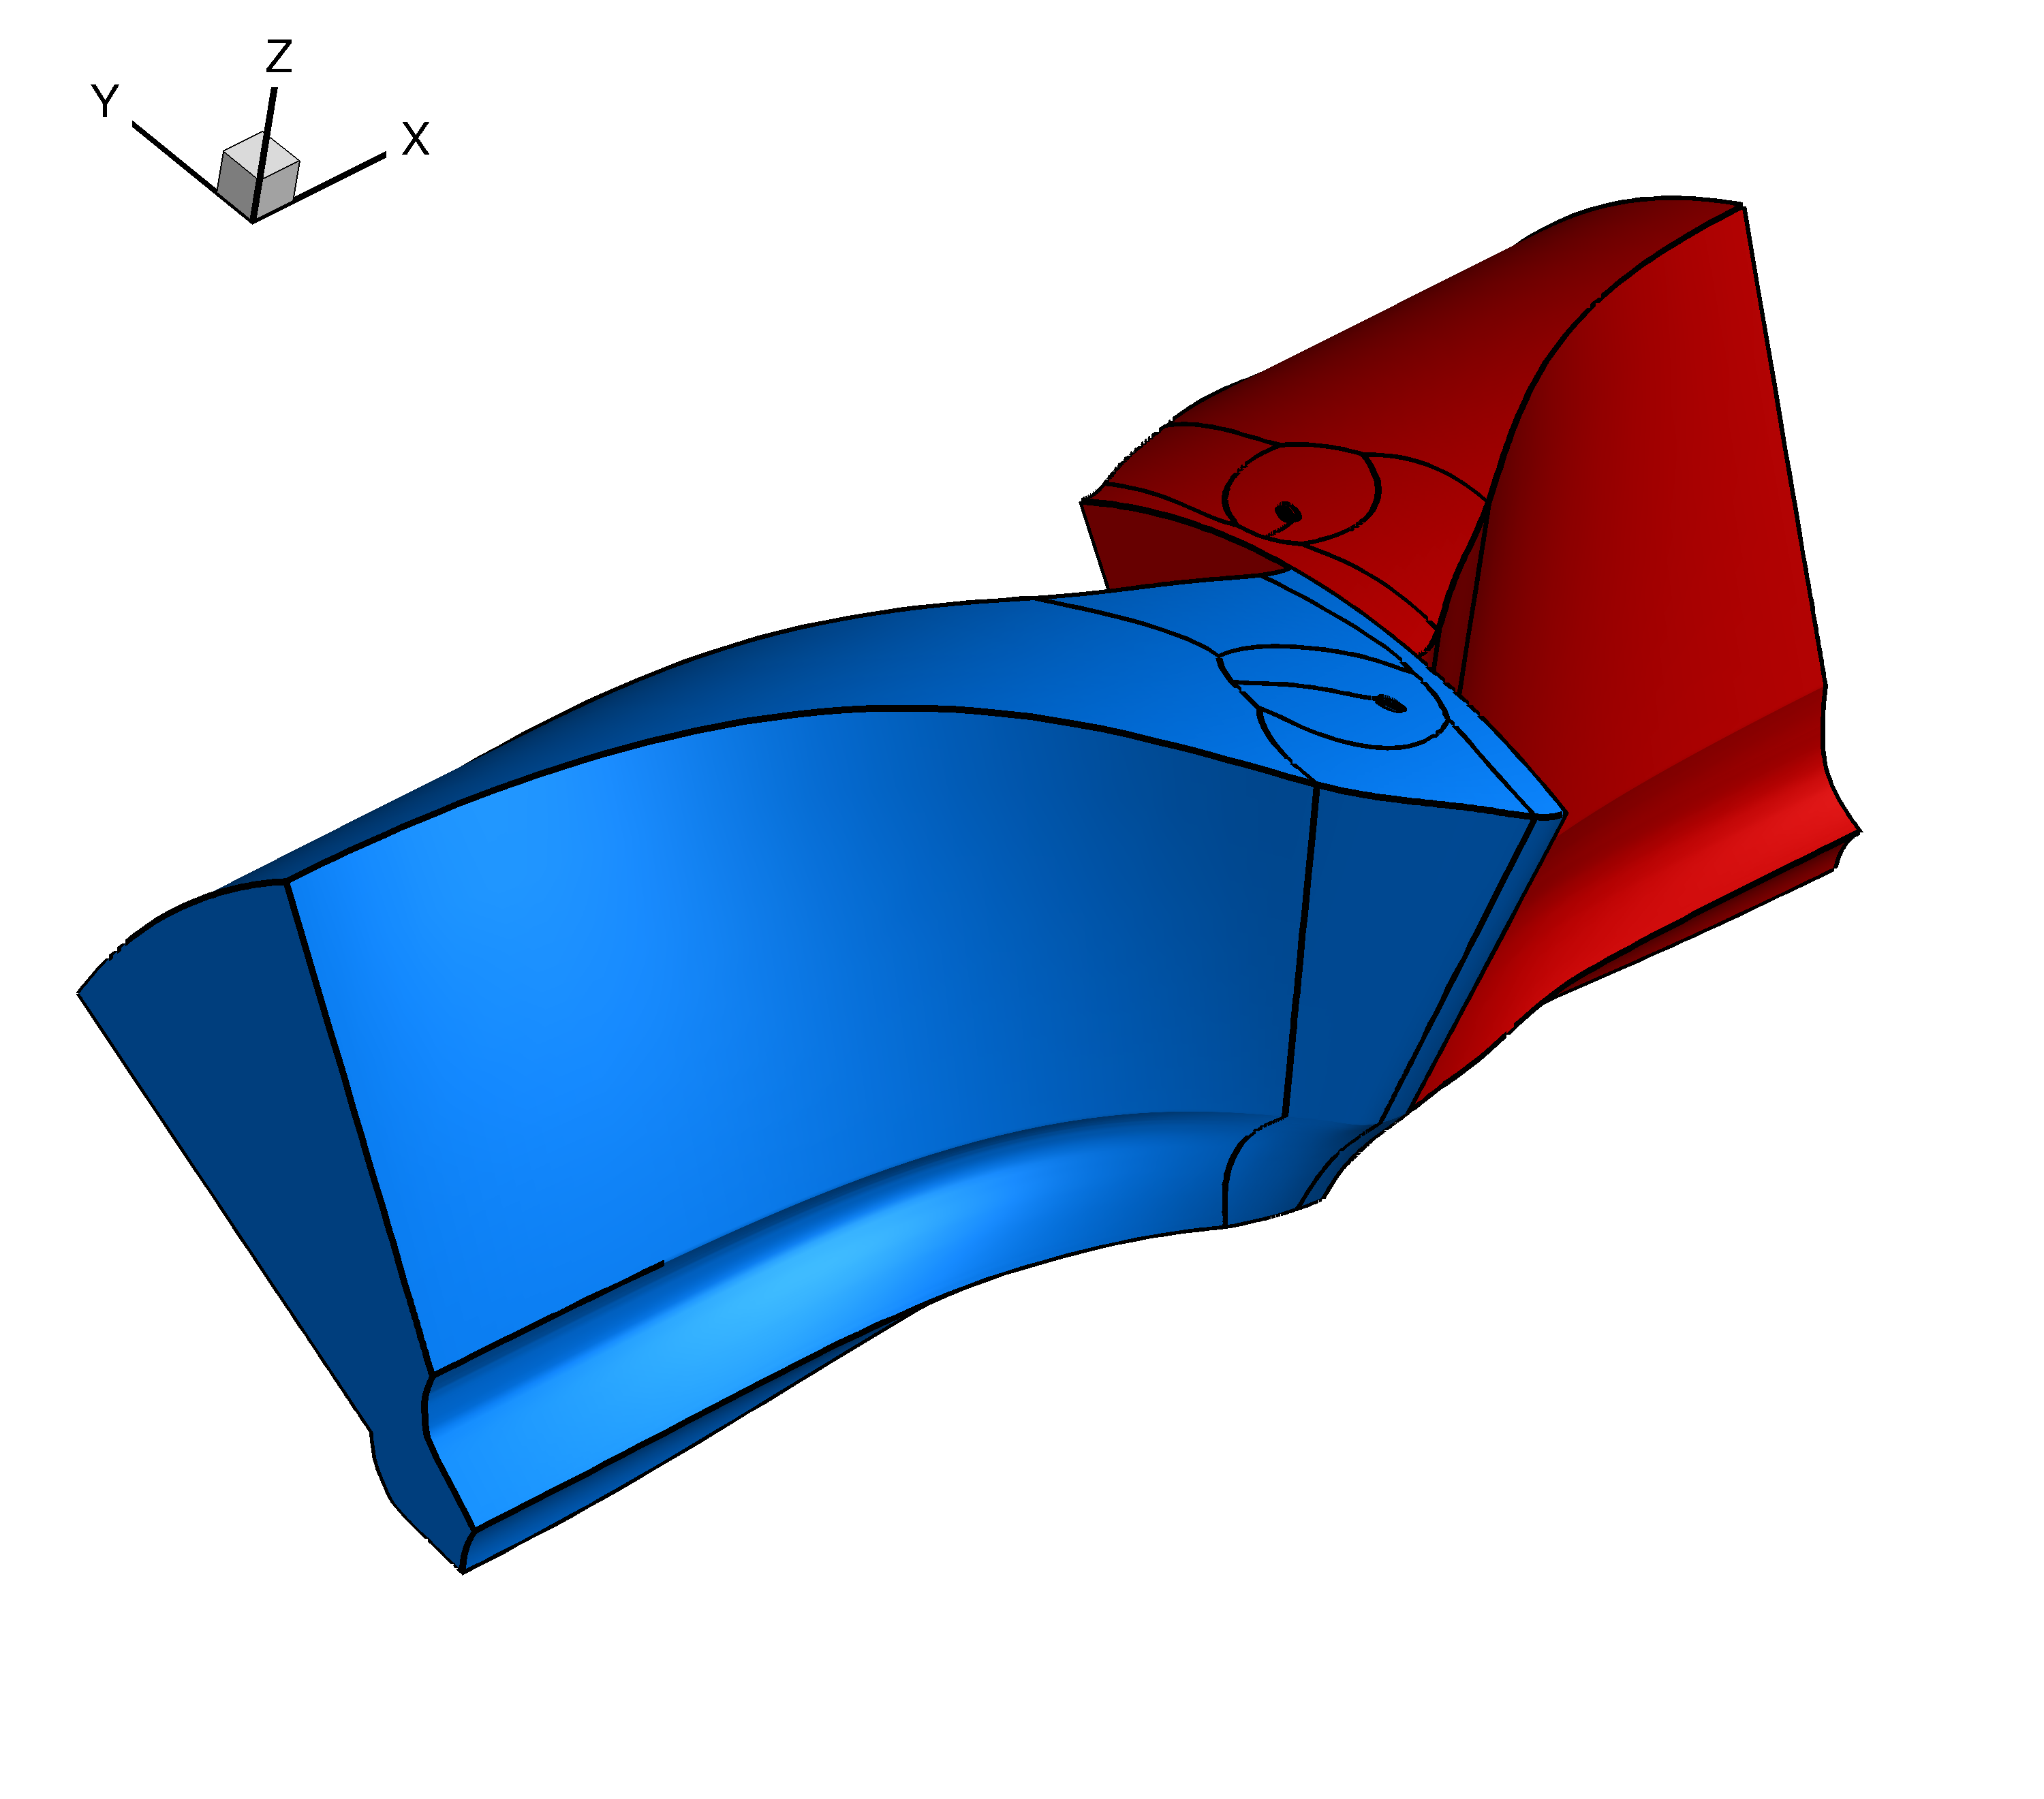
\includegraphics[height=.4\textwidth]{dream_mesh.png}}
  \subfigure[detailed topology with number of grid points]{
    \label{fig:dream_ls_mesh}
    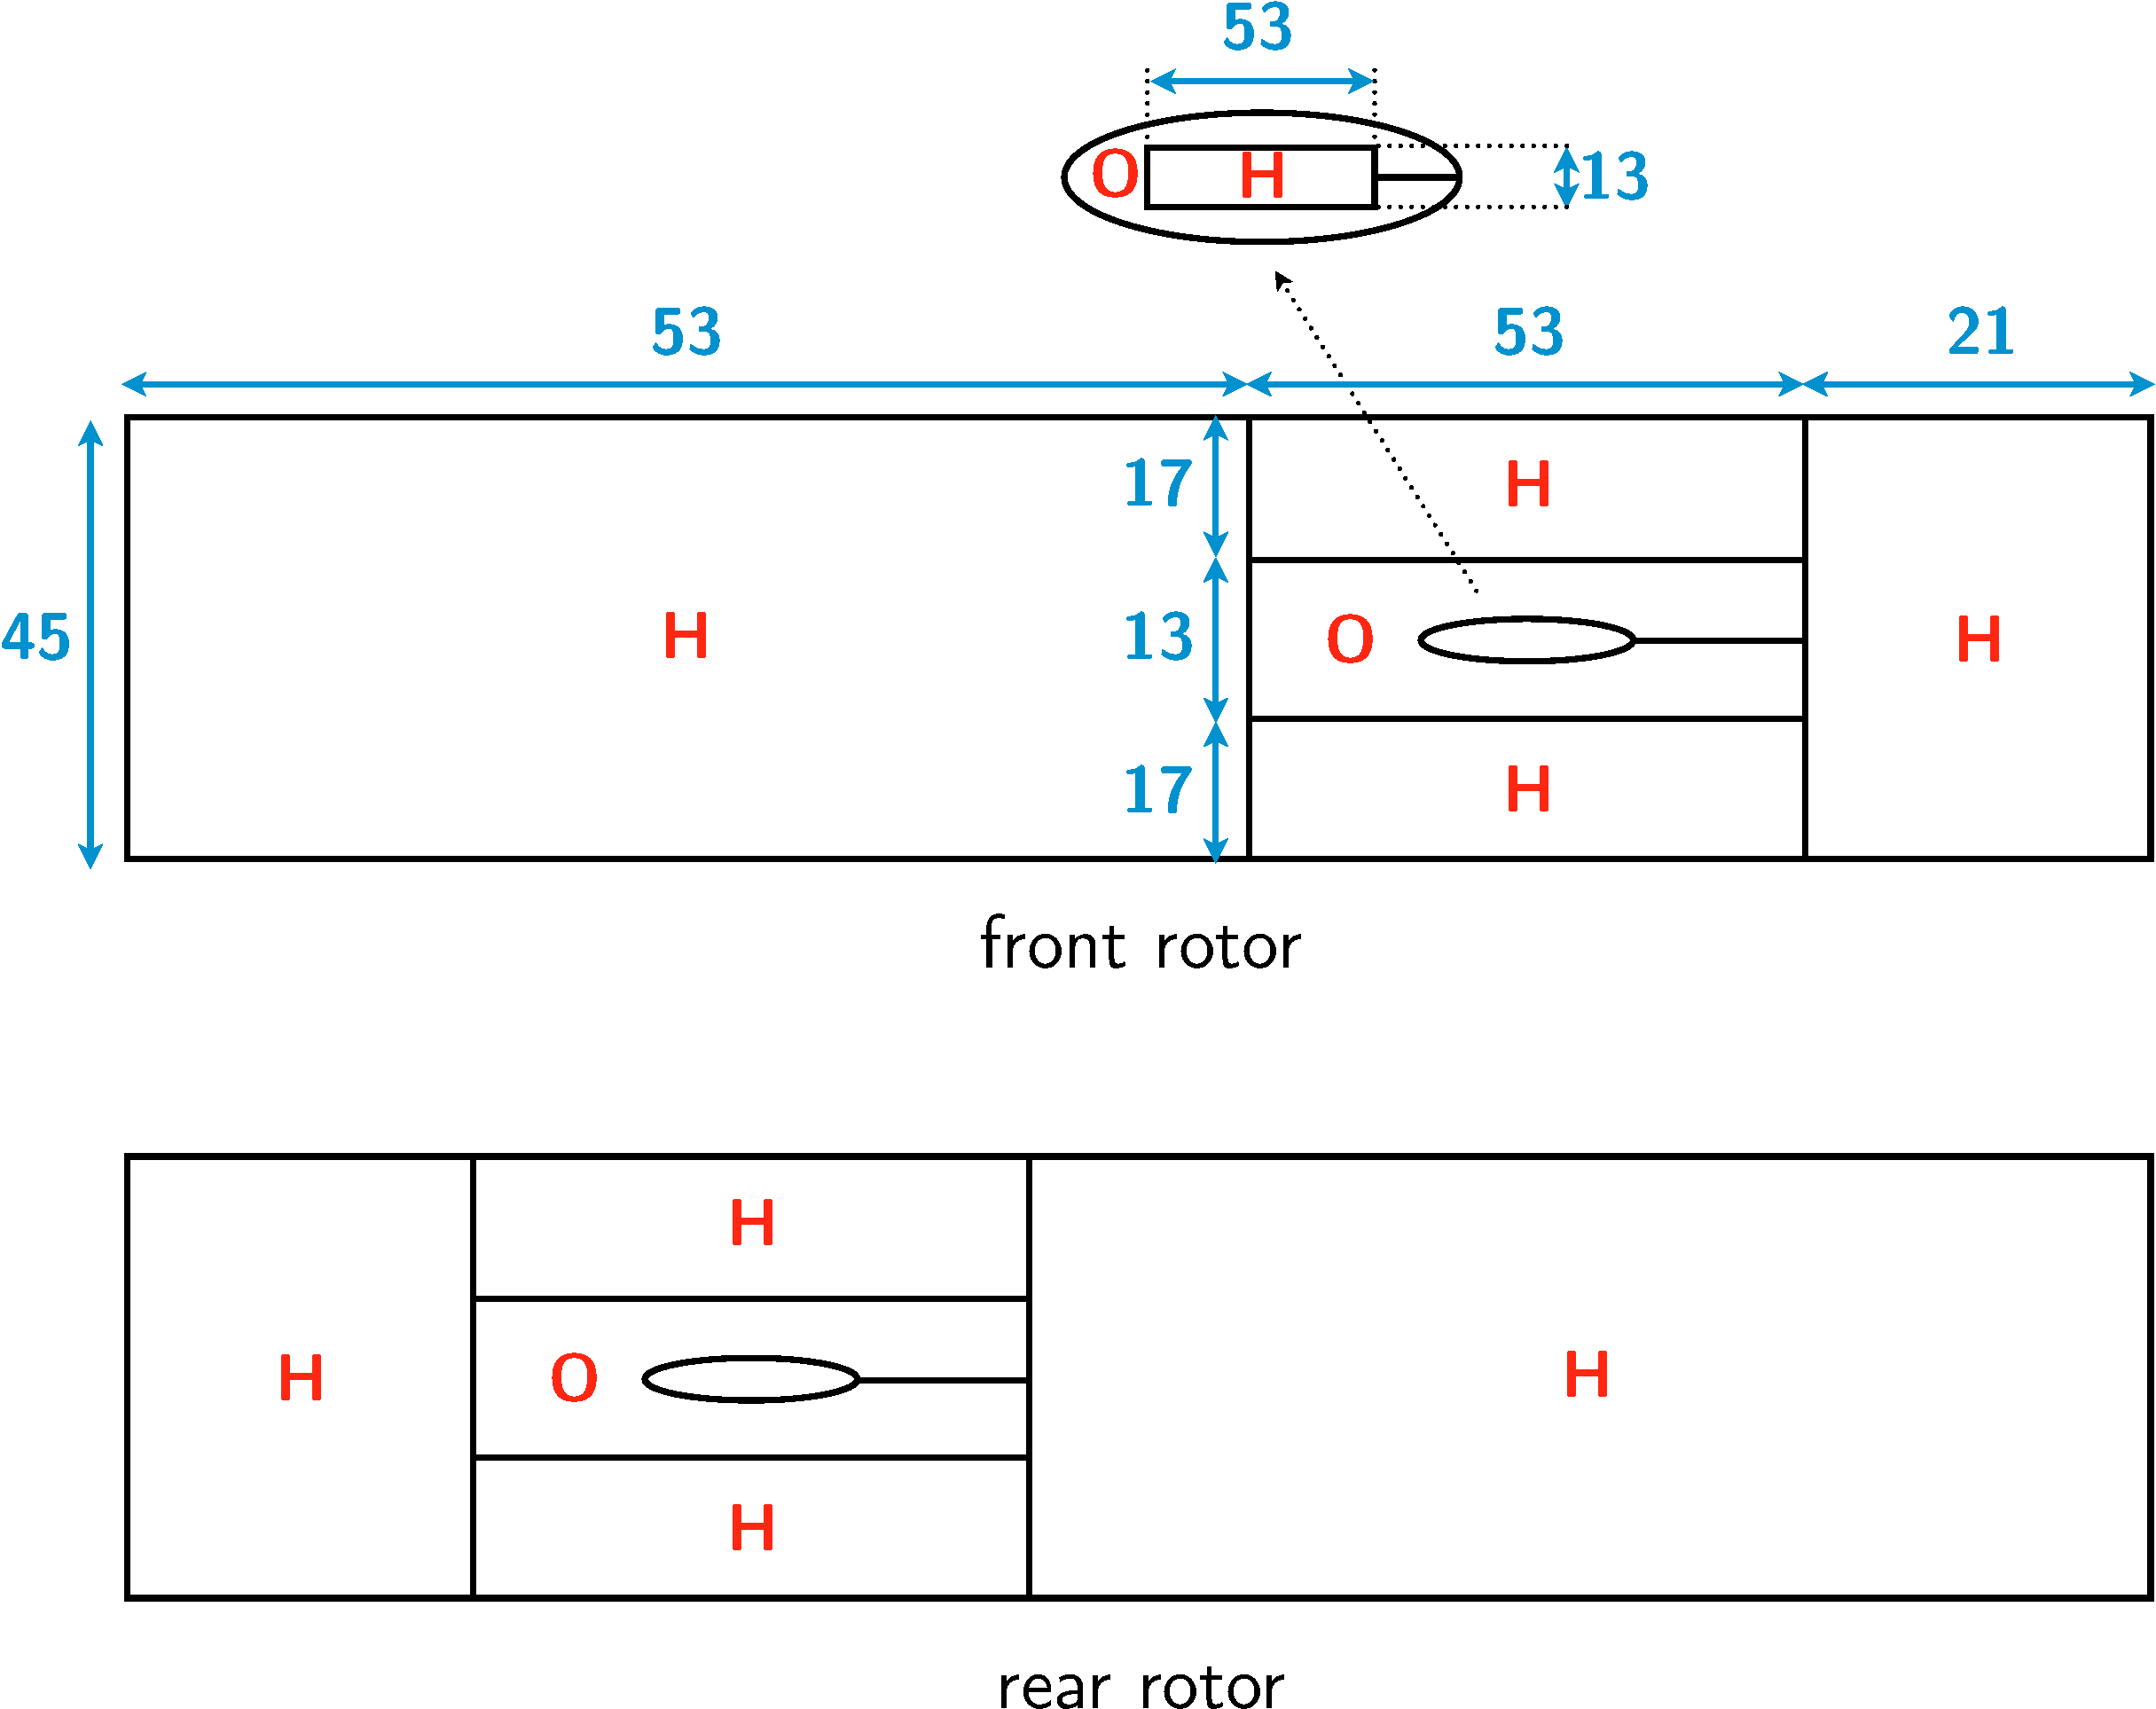
\includegraphics[height=.4\textwidth]{dream_ls_mesh.pdf}}
  \caption{Low-speed isolated configuration mesh topology.}
\end{figure}
The number of grid points is reported in 
Figure~\ref{fig:dream_ls_mesh} for a blade-to-blade section. 
129~points discretize the blade, 45~the pitch and 181~the radial
extent, among which~101 for the blade height. 
The same number of grid points is used for the front
and the rear rotor blades. 
Finally, the total number of grid points is almost $5$ million, which
is in the mid-range of the literature 
values~\cite{Stuermer2008,Bechet2011,
Francois2013,Zachariadis2011,Peters2012}.

As a CROR is not shrouded, a sufficiently large
far-field domain is taken to ensure a minimum influence
of the far-field boundary conditions on the results.
The computational domain is schematically reproduced 
in Figure~\ref{fig:dream_farfield}.
The radial extent is $3D$ while the axial one is $3.5D$, with
$D$ being the diameter of the front rotor.
In the literature, 
\citet{Peters2012} consider an axial extent of $7.5D$
with a radial extent of $4D$ while \citet{Zachariadis2011}
consider $2.5D$ and $3.6D$, respectively. We are thus in 
the mid-range of the values taken in the literature.
\begin{figure}[htp]
  \centering
  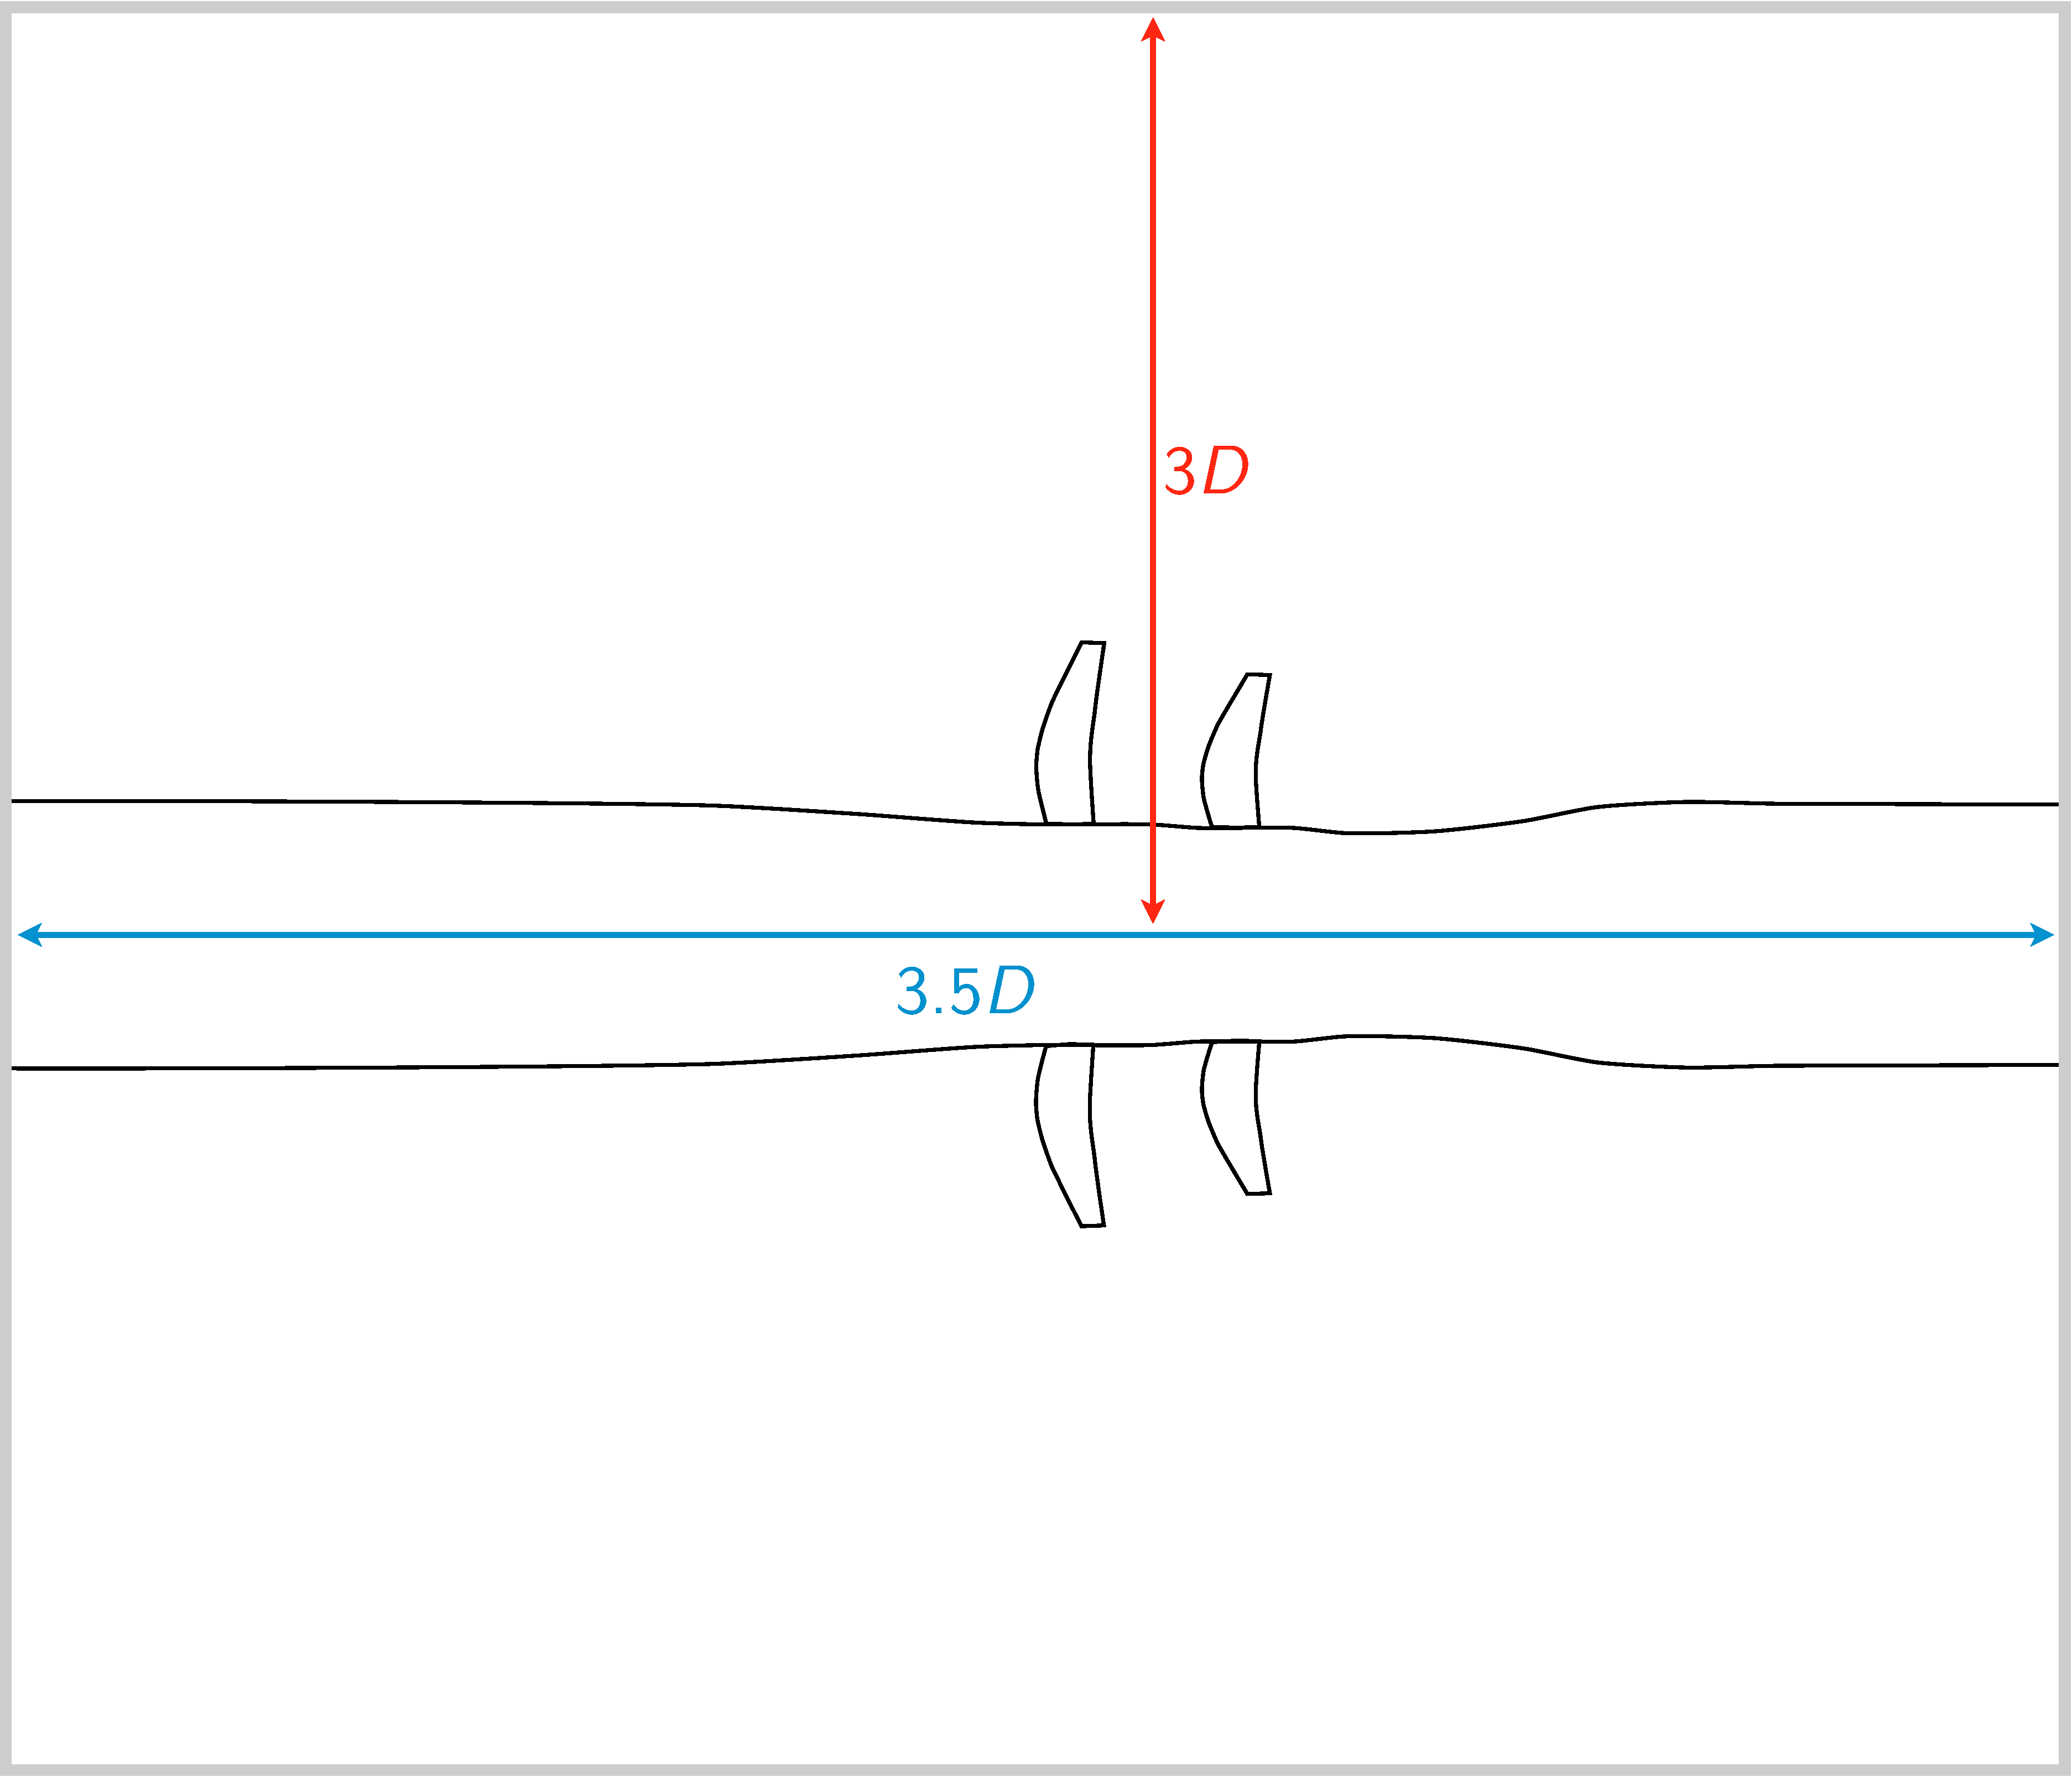
\includegraphics[width=.4\textwidth]{dream_farfield.pdf}
  \caption{Low-speed isolated configuration far-field domain and boundary conditions.}
  \label{fig:dream_farfield}
\end{figure}
As highlighted by the underlined text in Figure~\ref{fig:dream_farfield},
the boundary conditions used here are: (i)~adiabatic walls
for the blades and the hub (or spinner), (ii)~constant
stagnation values for the far-field, (iii)~periodic
or phase-lagged boundary conditions 
for the azimuthal boundaries of the channel
and (iv)~mixing-plane or sliding mesh interface for the
rotors interface depending on the type of computation (steady or unsteady).
In this case,
the mesh stems from literature and industrial best
practices and will not be assessed.

Turbulence is modeled using the one-equation model of
\citet{Spalart1992}.  Roe's scheme~\cite{Roe1981} along with a 
second-order MUSCL extrapolation 
is used to compute the convective fluxes.
The maximum CFL number is set to~10 for the steady 
computations and to~5 for the unsteady simulations.

For the aeroelastic computations shown in
Sec.~\ref{sec:dream_ls_ael_results}, 
the aeroelastic module~\cite{CIDugeai2011} 
of the \textit{elsA}~\cite{Cambier2013} CFD code is used.
Again, only a one-blade passage domain is meshed.
Phase-lag boundary conditions are therefore used
and each computed frequency is associated to one phase-lag
as shown by \citet{ThesisGuedeney}.
For the aeroelastic modes, 
four nodal diameters are considered, corresponding to Inter-Blade
Phase Angles (IBPA) of: $[-60^\circ, -30^\circ, 30^\circ, 60^\circ]$. 
The aeroelastic coupling is considered to be linear (weak-coupling
approach), therefore a very small amplitude of the mode is applied
and the fluid response is analyzed.
In this work, the two frequencies 
have a different physical meaning. In fact, while the blade passing frequency
has been shown to convey the main flow physics (potential effects, wakes, 
tip vortices, to name but a few), the aeroelastic frequency is more likely
to influence the near blade wall flow field. In fact, as recalled
previously, the amplitude of vibration is kept very small,
yielding a local influence of the blade vibration.
Therefore, it seems reasonable to use the "cross grid"
truncation pattern (see Sec.~\ref{par:choice_of_frequencies}).
Thus, the harmonic balance computations are run with
five frequencies in total. In the rear rotor,
the harmonics of the front rotor blade passing frequency
are chosen. In the front rotor, the first frequency is the
frequency associated to the vibration of the blade and the
remaining ones are the harmonics of the rear rotor blade 
passing frequency.
The time instances are automatically chosen using the OPT
algorithm (see Sec.~\ref{sec:algo_opt}) which leads to 
a condition number always lower than $1.1$ which ensure
the stability of the computations.

\paragraph{Influence of the spatial discretization}
\label{sub:dream_ls_spatial_discretization}

To assess the influence of spatial discretization, two 
space discretization schemes are used to simulate this low-speed CROR configuration.
These schemes are the \citet{Jameson1981} scheme (JST) with artificial
viscosities $\kappa_4 = 0.016$, $\kappa_4 = 0.032$, $\kappa_4 = 0.064$
and $\kappa_2$ equal to $0.5$. In addition to this scheme, we consider
Roe's scheme~\cite{Roe1981} without MUSCL extrapolation (Roe~1),
and with second-order (Roe~2) or third-order (Roe~3) 
MUSCL extrapolations.

Convergence histories of the different computations are shown 
in Figure~\ref{fig:dream_ls_space_scheme_residual}
for the four schemes. The convergence is not 
very good. Only the Roe~1 and Roe~2 spatial schemes give 
a convergence that has an acceptable slope. On the contrary,
the JST with $\kappa_4 = 0.016$ diverges and hardly converges
when using different values of the artificial viscosity
parameters. The higher the
viscosity parameter $\kappa_4$ of the JST scheme, the better
the convergence. Exceeding $\kappa_4 = 0.064$ should
warn us that something might be wrong with the computation.
As stated previously, this can be attributed to the range of Mach
number in which this low-speed configuration operates
or to any stiff flow features as for instance flow separation.
\begin{figure}[htp]
  \centering
  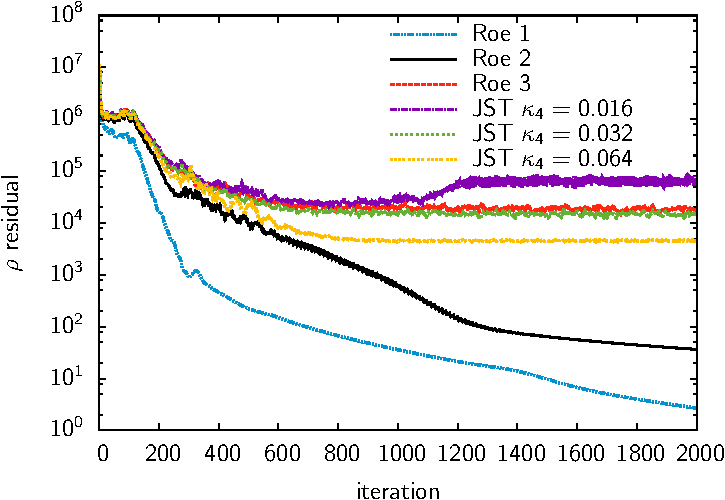
\includegraphics[width=.5\textwidth]{SPACE_SCHEME_DIFF_LS_RESIDUALS.pdf}
  \caption{Low-speed isolated configuration: convergence of the
  steady computations using different spatial schemes.}
  \label{fig:dream_ls_space_scheme_residual}
\end{figure}

To further differentiate the spatial schemes, 
the steady results for the similarity coefficients are reported
in Figure~\ref{fig:dream_ls_space_scheme_coeff} for all spatial scheme, 
except the diverging JST~$\kappa_4 = 0.016$ computation.
Arbitrarily, the results are normalized by the Roe~2 values.
The Roe~2, Roe~3, and the JST scheme with different choices
of the dissipation coefficients give equivalent
similarity coefficients as the difference is smaller than 1~\%.
In opposite, the first-order upwind scheme (Roe~1) gives a 5~\%
difference for both the traction coefficient $C_T$ and the efficiency $\eta$.
Cross-comparing these results with the convergence of the computations
reported in Figure~\ref{fig:dream_ls_space_scheme_residual}, the Roe~2
scheme is kept for the following as it gives both a good convergence
of the residuals and consistent similarity coefficients.
\begin{figure}[htp]
  \centering
  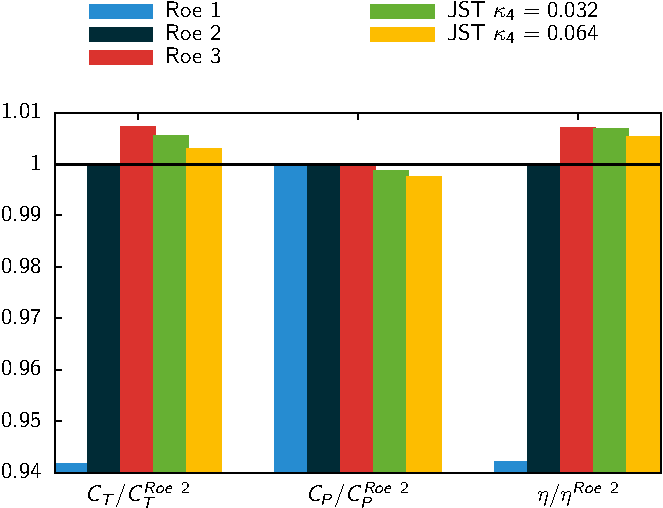
\includegraphics[width=.5\textwidth]{SPACE_SCHEME_DIFF_LS_COEFF.pdf}
  \caption{Low-speed isolated configuration: convergence of the 
  similarity coefficients using different spatial schemes.}
  \label{fig:dream_ls_space_scheme_coeff}
\end{figure}

